\documentclass[headings=normal]{ctexart}  % 对应 article 文档类，ctexbook/ctexrep 对应 book/report
\usepackage{graphicx}
\pagestyle{plain} % 使用简单页眉样式，只显示页码
\title{层次分析法解析} % 标题
\author{作者：彭奥祺} % 作者
\date{\today} % 日期

\begin{document}
\maketitle % 生成标题

\section{创建表格} % 章节

\begin{figure}[htbp]
    \centering
    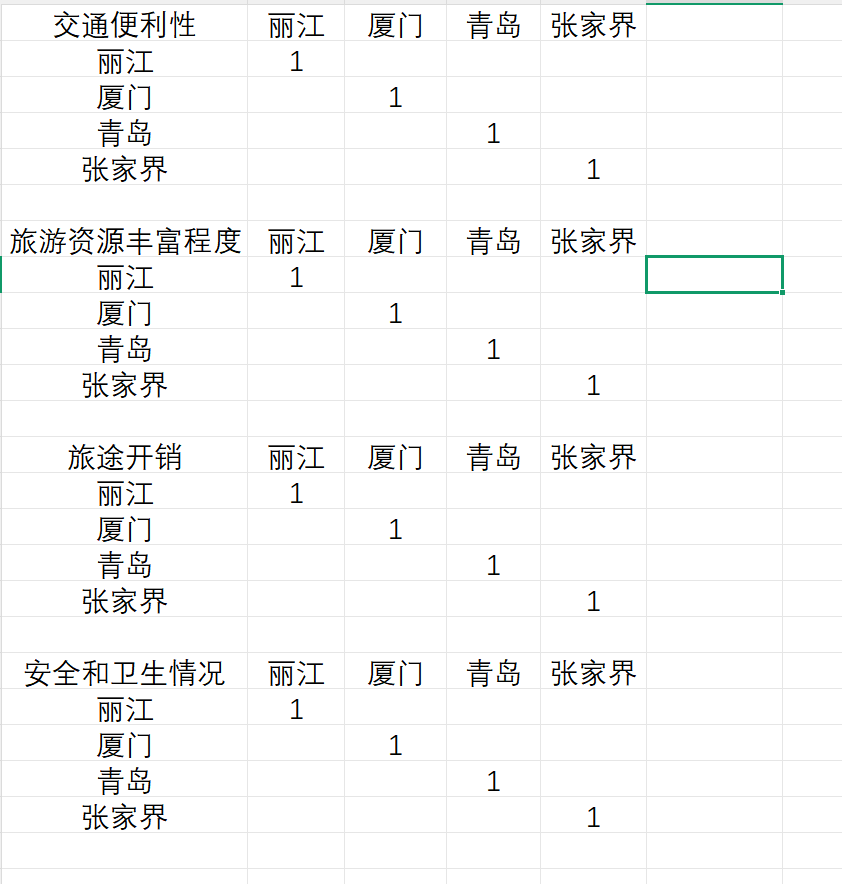
\includegraphics[width=0.8\linewidth]{QQ20260304-190056.png}
    \caption{层次分析法表格}
    \label{fig:table}
\end{figure}

\section{利用层次分析法填充表格}

\begin{enumerate}
    \item 问AI获得数据
    \item 填充数据
    \item 初步检查数据
\end{enumerate}

\begin{figure}[htbp]
    \centering
    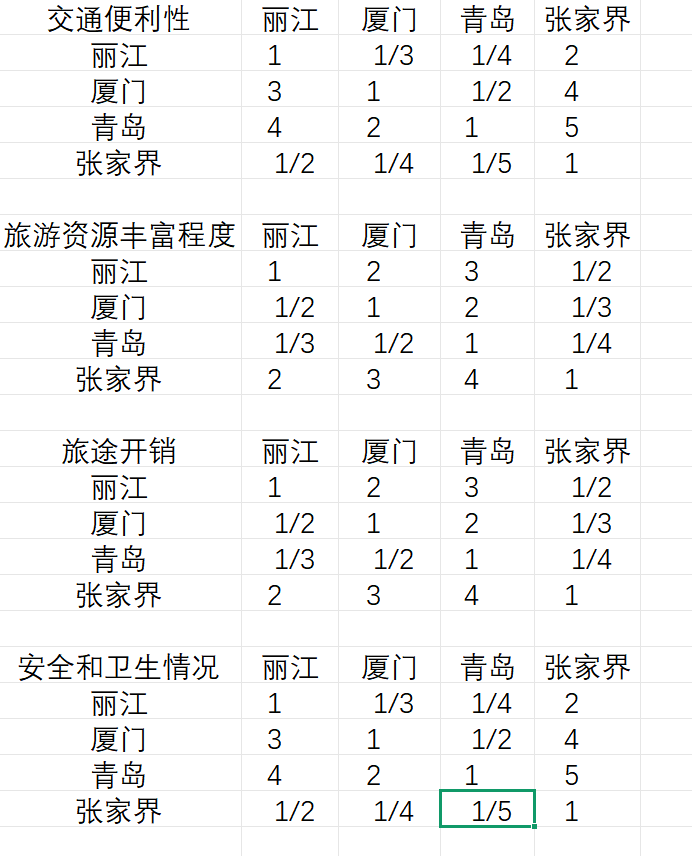
\includegraphics[width=0.8\linewidth]{QQ20260304-203319.png}
    \caption{填充数据}
    \label{fig:table}
\end{figure}

\section{一致性检验}

\begin{enumerate}
    \item 列求和
    \item 归一化
    \item 横求和
    \item 横数据归一化->得权重
\end{enumerate}

过程见一致性检验.md

\section{获得不同指标的权重}

\begin{enumerate}
    \item 同上列出指标的判断矩阵
    \item 进行一致性检验
    \item 获得不同指标的权重
\end{enumerate}

见获得指标权重.md

\section{计算得分}

见计算得分.md

\end{document}